\begin{frame}{Lifting Framework 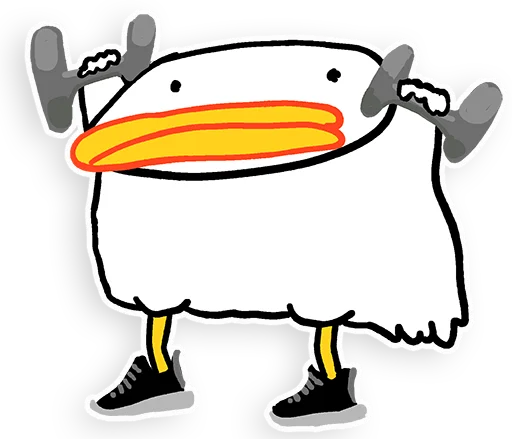
\includegraphics[scale = 0.04]{pics/utia-lift.png}}

    \centering

    Resolution proof lower (or upper bounds). [GMR\textcolor{red}{S}, 25]

    \vspace{0.1cm}
    \tikz{
        \node[scale = 0.45, fancy-arrow = {black}{LEIred!40!white}{LEIblue}] (a) {};
        \node[right = 1cm] at (a) {[Pudlak, 00]};
        \node[right = 3cm] at (a) {};
        \node[left = 3cm] at (a) {};
    }
    
    \vspace{0.1cm}
    Resolution game for $\Search$.

    \vspace{0.1cm}
    \tikz{
        \node[scale = 0.45, fancy-arrow = {black}{LEIred!40!white}{LEIblue}] {};
        \node[right = 1cm] at (a) {[GGK\textcolor{red}{S}, 18]};
        \node[right = 3cm] at (a) {};
        \node[left = 3cm] at (a) {};
    }
    
    \vspace{0.1cm}
    \alert{Dag-like} communication protocol for ``lifted'' $\Search$.

    [Razborov, 95; Pudlak, 10; \textcolor{red}{S}, 17]

    \vspace{0.1cm}
    \tikz{
        \node[scale = 0.45, fancy-arrow = {black}{LEIred!40!white}{LEIblue}] {};
        \node[right = 1cm] at (a) {[Razborov, 90]};
        \node[right = 3cm] at (a) {};
        \node[left = 3cm] at (a) {};
    }
    
    \vspace{0.1cm}
    \alert{Dag-like} communication protocol for the KW relation for a function $f_{\text{Brackets}}$.

    \vspace{0.1cm}
    \tikz{
        \node[scale = 0.45, fancy-arrow = {black}{LEIred!40!white}{LEIblue}] {};
        \node[right = 1cm] at (a) {[KW 88; R 95; P 00; \textcolor{red}{S}, 17]};
        \node[right = 5cm] at (a) {};
        \node[left = 5cm] at (a) {};
    }

    \vspace{0.1cm}
    Monotone circuits for $f_{\text{Brackets}}$.
    
\end{frame}

\begin{frame}{$\KWm$ Relation [Karchmer, Wigderson 90]}
    Let $U, V \subseteq \{0, 1\}^{n}$ and $U \cap V = \emptyset$.

    \vspace{0.1cm}
    $\KWm$:
    \begin{itemize}
        \item Alice gets $u \in U$, Bob gets $v \in V$;
        \item goal: find $i$ such that $u_i = 1 \land v_i = 0$.
    \end{itemize}

    \pause

    \begin{theorem}[Karchmer, Wigderson 90]
        $\mathrm{F\text{-}Size}(f) \le S$ $\Leftrightarrow$ communication protocol
        for $\KWm$ of size $S$, where $U \coloneqq f^{-1}(1), V \coloneqq f^{-1}(0)$.
    \end{theorem}

    \pause
    \begin{theorem}[Razborov 95; Pudlak 10; S 17]
        $\mathrm{C\text{-}Size}(f) \le S$ $\Leftrightarrow$ communication \alert{dag}
        for $\KWm$ of size $S$, where $U \coloneqq f^{-1}(1), V \coloneqq f^{-1}(0)$.
    \end{theorem}
\end{frame}



\begin{frame}{$\KWm$ is a ``Complete Relation''}

    \begin{itemize}
        \item $\mathcal{S} \subseteq U \times V \times \mathcal{O}$;
        \item define $F_{\mathcal{S}}\colon \{0, 1\}^m \to \{0, 1\}$ such that
            $\DCC(\KWm[F_{\mathcal{S}}]) = \DCC(S)$.
    \end{itemize}

    \pause

    \vspace{-0.2cm}
    \begin{center}
        \tikzstyle{ops} = [alt=<{#1}>{opacity = 1}{opacity = 0}]

\begin{tikzpicture}
    \draw[thick, rounded corners = 2pt] (0, 0) rectangle (4, 3);
    \node at (-0.3, 1.5) {$U$};
    \node at (5, 1.5) {};
    \node at (2, 3.3) {$V$};

    \draw[red!30, fill = red!10, rounded corners = 3pt] (0.3, 0.1) rectangle (1, 2.9)
        node[midway, red!80] {$1\colon o_i$};
    \draw[green!50!black, fill = green!30, rounded corners = 3pt, opacity = 0.5] (0.5, 0.4) rectangle
        (3.5, 0.9) node[midway, green!20!black] {$2\colon o_j$};
    \draw[blue!50!black, fill = blue!30, rounded corners = 3pt, opacity = 0.5] (0.7, 2) rectangle
        (3.4, 2.85) node[midway, blue!20!black] {$3\colon o_k$};
    \draw[ops = 3, very thick, red] (-1, 0.5) -- (5, 0.5);
    \draw[ops = 4, very thick, red] (3, -0.5) -- (3, 3.5);
\end{tikzpicture}
    \end{center}

    \pause
    $F_{\mathcal{S}}(1, 1, 0, \dots) \coloneqq 1$\pause, ~~~$F_{\mathcal{S}}(1, 0, 0, \dots) \coloneqq 0$

    \pause
    \begin{lemma}
        $\DCC(\KWm[F_{\mathcal{S}}]) = \DCC(S)$.
    \end{lemma}

    \pause
    \putpos{250}{110}{
\includegraphics[scale = 0.1]{pics/utia-think.png}}

\end{frame}



\begin{frame}{Lifting (informal) [Garg, G\"{o}\"{o}s, Kamath, S 18]}


    \begin{itemize}
        \item Function $g$ is carefully chosen!
    \end{itemize}

    \vspace{1cm}
    \begin{center}
        \alert{$\exists$} Resolution proof for $\varphi$ of width $w$ and depth $d$.

        $\Updownarrow$
        
        \alert{$\exists$} dag protocol for $\Search_{\varphi} \circ g$ of size $n^w$ and depth $\poly(n)
        \cdot d$.
    \end{center}

\end{frame}